\documentclass[9pt]{beamer}

\usetheme[{titleformat plain}=smallcaps,
           titleformat title=smallcaps,
           titleformat subtitle=regular,
           titleformat section=smallcaps,
           titleformat frame=smallcaps,
           numbering=fraction,
          ]{metropolis}
\usepackage{appendixnumberbeamer}
\geometry{paperwidth=213.3mm,paperheight=120mm}

\usepackage{../_style/common}
\usepackage{../_style/defs}
\usepackage{emoji}

\graphicspath{{pictures/}{../_pictures/}}

\title{Project Life-cycle}
\subtitle{
    \itshape
    from prototype to scaling
}
\date{October, 2022}
\author{Alessandro Candido}
\titlegraphic{
    \vfill\vspace*{250pt}
    \includegraphics[height=1cm]{../_logos/unimi_logo.png}\hfill
    \includegraphics[height=1cm]{../_logos/infn_logo.png}\\
}

\begin{document}

\maketitle

\setlist[description]{font=\quad\normalfont\bfseries\scshape\space}
\metroset{block=fill}


\begin{frame}{Who am I?}
    \begin{columns}
        \begin{column}{0.5\textwidth}
            I am a \textbf{PhD student} in \textbf{HEP theory}, about to
            finish.\newline

            Since my Master I have spent a significant part of my research
            working on \alert{\textbf{software projects}}, with an increasing
            number of collaborators.\newline

            \partitle{References}\newline

            Now, as part of \nnpdf{}, I had to work and organize projects with
            $\order{10}$ developers -- not incredibly many, but already
            \textit{\textbf{challenging}}.\newline

            Moreover, personal projects driven me to explore beyond the
            boundaries of what is useful for physics.
            With less \sout{pressure} needs you can explore more\dots but often
            not as deep.\newline

            \partitle{My Goal}\newline

            I am not here to teach, but just to \textbf{share my experience}.
            This is compliant with the references.
        \end{column}
        \begin{column}{0.5\textwidth}
            \begin{figure}
                \centering
                \includegraphics[width=0.5\textwidth]{mygh}
            \end{figure}
        \end{column}
    \end{columns}
\end{frame}

\begin{frame}{The Role of Trade-offs}
    \begin{columns}
        \begin{column}{0.5\textwidth}
            \vspace*{20pt}
            \begin{center}
                \itshape\bfseries 
                There are no absolute truths.
            \end{center}
            \begin{flushright}
                \itshape
                -- is this an absolute truth? \emoji{thinking-face}
            \end{flushright}

            \vspace*{10pt}
            In a sense, problems might look similar, even when they are not
            that much\dots
            \vspace*{20pt}
            
            \begin{figure}
                \centering
                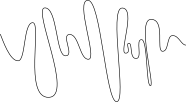
\includegraphics[width=\textwidth]{solution}
                \caption{
                    Artistic view of the solution function, over the space of
                    problems.
                }
            \end{figure}
        \end{column}
        \begin{column}{0.5\textwidth}
            So, better to know many possible solutions, and always consider
            multiple alternatives.

            \vspace*{10pt}
            \begin{figure}
                \centering
                \includegraphics[width=0.6\textwidth]{balancing}
            \end{figure}
            \vspace*{10pt}

            Moreover
            \href{https://en.wikipedia.org/wiki/All_that_glitters_is_not_gold\#In_popular_culture}{\enquote{All
            that is gold does not glitter}}, not all good solutions are
            manifest.
        \end{column}
    \end{columns}
\end{frame}

\section{Starting Point}

\begin{frame}{The Problem}
    \begin{columns}
        \begin{column}{0.5\textwidth}
            
        \end{column}
        \begin{column}{0.5\textwidth}
            
        \end{column}
    \end{columns}
\end{frame}

\section{first section}

\begin{frame}{Template}
    \begin{columns}
        \begin{column}{0.5\textwidth}
            
        \end{column}
        \begin{column}{0.5\textwidth}
            
        \end{column}
    \end{columns}
\end{frame}

\begin{frame}{Filled Template}
    \begin{columns}
        \begin{column}{0.5\textwidth}
            \lipsum[1]
        \end{column}
        \begin{column}{0.5\textwidth}
            \lipsum[1][1-2]

            \begin{figure}
                \centering
                \begin{tcolorbox}[width=0.5\textwidth,size=tight,sharpish corners,boxrule=0mm]
                    \includegraphics[width=\textwidth]{balancing}
                \end{tcolorbox}
            \end{figure}

            \lipsum[1][3-4]
        \end{column}
    \end{columns}
\end{frame}

\begin{frame}{Another Slide}
    \begin{tcolorbox}[size=tight,sharpish corners,boxrule=0mm]
        \includegraphics[width=0.5\textwidth]{poetry-vs-pipenv}
    \end{tcolorbox}
\end{frame}

\begin{frame}[standout]
    Thanks for your attention!
\end{frame}

\appendix

\begin{frame}{Appendix Slide}
\end{frame}

\end{document}
